\documentclass[12pt, a4paper]{jreport}

\usepackage[driver=dvipdfm]{geometry}
\usepackage[dvipdfmx]{graphicx, color}
\usepackage{here}
\usepackage{plext}
\usepackage{times, mathptmx}
\usepackage{longtable}
\usepackage{colortbl}
\usepackage{tabularx}
\usepackage{enumerate}
\usepackage{comment}
\usepackage{url}
\usepackage{lscape}
\usepackage{multirow}
%\usepackage{otf}

\setlength{\voffset}{0.5truecm}
\setlength{\headsep}{2truecm}
\setlength{\oddsidemargin}{7.0truemm}
\setlength{\evensidemargin}{-5.5truemm}
\setlength{\topmargin}{-1truecm}
\setlength{\footskip}{25truemm}
\setlength{\textwidth}{15truecm}
\setlength{\textheight}{22truecm}
\makeatletter
\makeatother

\begin{document}
    \title{プログラムコードの複雑さの防止効果が高い\\システム開発上の要素の検討\\Consideration of view points\\that contribute to the prevention of\\program code complexity in system development}
    \author{指導教員:山川 広人\\
    公立 千歳科学技術大学 理工学部\\
    情報システム学科 山川研究室\\
B2201400 須藤 真由}
\date{\today}

\maketitle
\pagenumbering{roman}
\tableofcontents
\chapter{序論}
\pagenumbering{arabic}

\section{背景}
複雑なプログラムコードがシステム開発上やプログラミング教育の上で障壁となることがある。平嶋ら\cite{haikei}は高等教育機関におけるプログラミング講義に苦手意識を持つ学習者に着目し,プログラミング学習者の認知負荷を減少させ、アルゴリズムの組み立て等の適切な部分に集中できるようにするためにカードを並べ替える方式の学習方法を提案した。社会的にもプログラムコードの複雑さに対する取り組みや議論は盛んである。株式会社サイバーエージェント\cite{CyberZ}では、新卒採用されたエンジニア向けにプログラムコードの品質に関する講義を行った。プログラムコードの品質を上げることでプログラムコードの可読性が向上し、速い開発スピード維持することができると説明している。開発スピードの速さは市場での競争力に影響を与えることにも言及している。また、松田\cite{kireina}はきれいなプログラムを継続的に記述していくために気を付けるべきことについてまとめており、その中で1つのメソッドが長くなることで発生する複雑さや、適切な命名を行うことで読みやすくなることについて述べている。プログラムコードの複雑さは学習やシステム開発をする上で問題となり得るため、システムの継続的な発展のためにも解決すべき課題であると捉えられている。
\\ 認知負荷に対する研究は高等教育機関におけるPBL学習(Ploject Based Learning)に対しても有用である。PBL学習には企業や地域のステークホルダーと連携し、数世代に亘ってプロジェクトを引継ぐことで成果物の発展や価値提供を行い続けるものがある。しかし、学生は複雑さを招かずにシステム開発をする知識や認知負荷を下げるという意識を必ずしも持ち合わせてはいないため、成果物として複雑なプログラムコードが出来上がることがある。その成果物を次の世代のプロジェクトが引き継ぐ際に、複雑なプログラムコードを読み解くことに時間がかかり問題解決に十分な時間を割くことができないことや、新たにプログラムコードを追加、変更した際に、さらに複雑なものにしてしまうことがある。PBL学習を効果的に行うためにも、複雑さの原因や複雑さを防止する方法について明らかにする必要がある。
\section{目的}
本研究では複雑さが防止されたプログラムコードの設計、開発方法を明らかにすることが目的である。また、ステークホルダーと継続的に価値共創を行っていくシステム開発プロジェクトを想定している。プログラムコードの複雑さが招かれる原因ははどこに存在しているかを分析し、どのような要素を取り入れることで複雑さを防止できるか、また複雑さが防止できていることをどのように確認できるか検討することで以下に示す2点のリサーチクエスチョンについて検証し、検討した要素や方法の有用性について考察を行う。
\begin{enumerate}
\item プログラムコードの複雑さの防止効果が高いシステム開発上の要素は何か
\item その要素がプログラムコードに
反映されているか評価する方法は何か
\end{enumerate}
\section{構成}
本論文は全6章で構成している。2章で関連している研究と本研究の位置づけについて述べる。3,4章でリサーチクエスチョン1について、複雑なプログラムコードの分析結果と改善案について述べる。5章でリサーチクエスチョン2について、評価方法の検討と結果、結果を踏まえた考察について述べる。6章では3,4,5章を踏まえ本研究の結論を述べる。
\chapter{先行研究と本研究の位置づけ}
\section{先行研究}
\subsection{}
\subsection{}
\section{本研究の位置づけ}
\chapter{複雑さの原因の分析と改善案の提案}
\section{研究の対象とするシステム}
プログラムコードの複雑さを招いている現状を分析し、複雑さの原因を分析する。複雑化したプログラムコードとして公立千歳科学技術大学で開発が進められてきた既存のシステムである「話しことばチェッカー」のプログラムコードを用いる。このシステムは文章を入力し検出ボタンを押すと文章内から話しことばを検出し、修正例と共に検出結果を示す文章校正システムである。
\\ このシステムは2018年度から開発が開始され、現時点で5年が経過している。開発は実システム開発を題材としたPBLの中で行われ、開発プロジェクトの責任者である話し言葉チェッカーのエキスパート教員(後述するドメインエキスパート)や、技術やスケジュール等をメンタリングするメンター教員は変わらないものの、求められる要件の定義や設計、それを実装として反映するプログラミングは年度ごとに異なるPBL参加学生が、前年度までの成果を引き継ぎながら開発を任される形で行ってきた。図3.1に、開発体制を示す。
\begin{figure}[H]
\centering
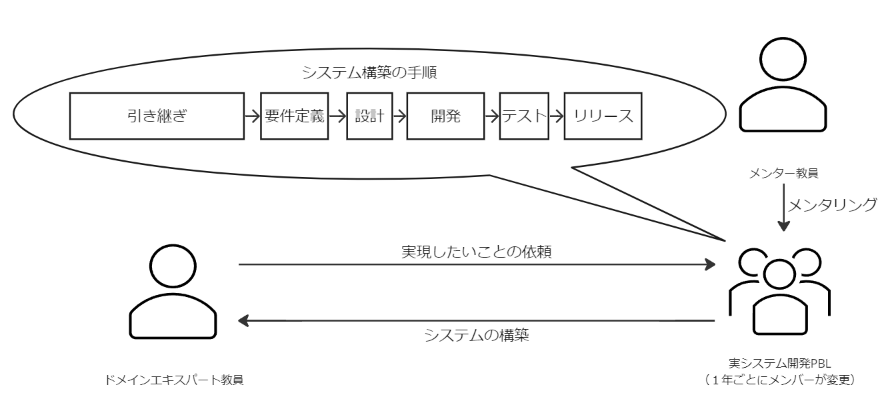
\includegraphics[width=1\linewidth]{image/taisyou1.1.png}
\caption{研究対象のシステムの開発体制}
\label{fig:enter-label}
\end{figure}
つまり、ドメインエキスパートが実現したいこと(話し言葉の検出・修正例の提示、およびそれらの年度ごとの改良)のシステム化に必要な要件の解釈や設計・実装はPBLの学生たちに任されている形であった。システムの規模は49クラス、2954行に上る。
\\ こうした中で、前年度の成果を引き継ぐ際、学生からはシステムが見かけ上正しく動作しているように見えるが、それを実現するプログラミングコードが難解であることが悩みの声として上がっていた。
\section{複雑さの原因の分析}
本研究は3.1で述べた状況からもシステムが5年間の開発の中で複雑化を引き起こしていると考え、プログラムコードを読み複雑さの原因となる問題点を以下の3つの観点から検討することにした。
\begin{enumerate}
\item どのような役割がどこに書かれているのか分からないコード
\item 開発者の独自の解釈を反映させたコード
\item どのような操作でどのような結果を示すのか分からないコード
\end{enumerate}
1について、以下に示した図3.1のプログラムコードのように1つのメソッドに多くの役割が含まれていること、話しことばの検出にまつわるメソッドがまとめて1つのクラスに書かれており、検出についての詳細な処理がどこに書かれているか探しにくい状態になっていた。
\begin{figure}[H]
\centering 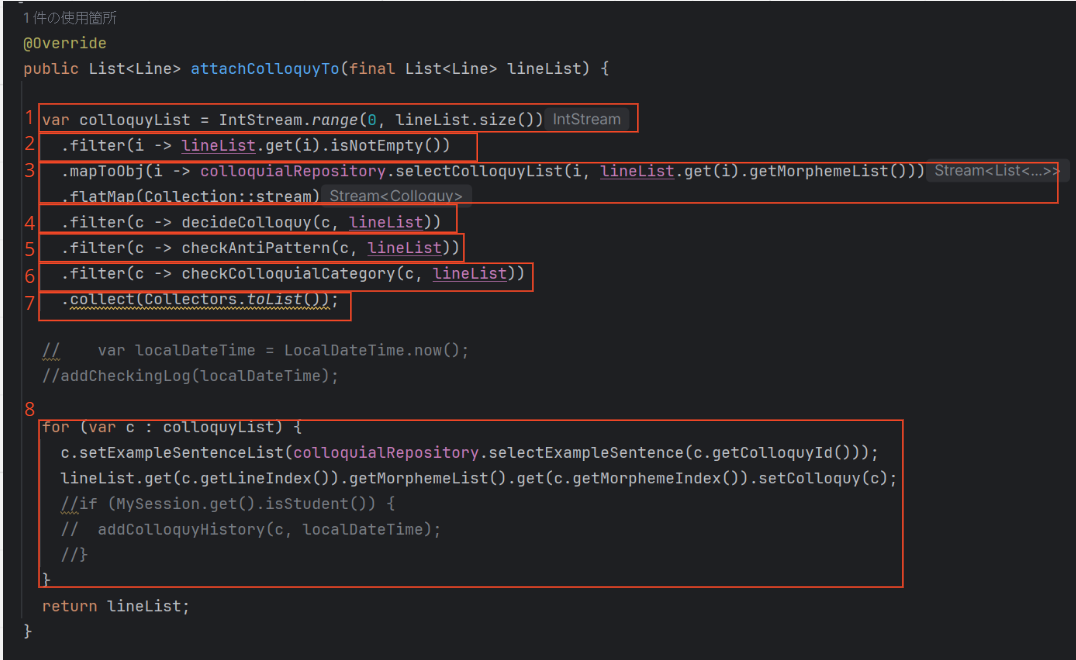
\includegraphics[width=1\linewidth]{image/genin1.1.png}
\caption{どのような役割がどこに書かれているのか分からないコードの例}
\label{fig:enter-label}
\end{figure}
2について、話しことばの検出の過程には形態素解析を行った後に形態素の前後関係を用いるものがあり、それらをカテゴリで分類し判断している。その中で、下に示す図3.2のクラス構造の赤丸で示したようにいくつか前の形態素を用いるものを"C2"や"Prefix"、「1つ」、「2つ」、「3つ」をドイツ語で"Eins"、"Zwei"、"Drei"等のように開発者独自の命名でプログラムコード上に示している。こういった命名の他、処理の内容や順番に開発者独自の考えが反映されていた。
\begin{figure}[H]
\centering
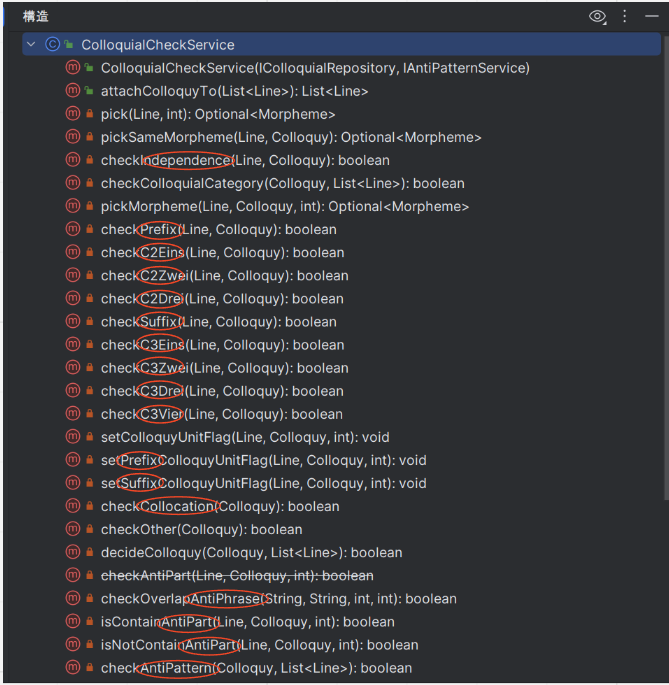
\includegraphics[width=1\linewidth]{image/genin2.1.png}
\caption{開発者の独自の解釈を反映させたコードの例}
\label{fig:enter-label}
\end{figure}
3について、このシステムがどのような操作でどのような結果を示すものなのか、どのような実装がされていればステークホルダーの要求を満たしているのか、確かめる手段が用意されていなかった。したがってこれまでのPBLではシステムを実際に動かし、結果に相違がないか目視で確認する方法でリリース前のテストを行っていた。
\section{複雑さの防止方法の提案}
プログラムコードの複雑さの原因に基づき、改善する方法として適切なモデリングとテストコードの整備が有効であると仮定して、リファクタリングを行いプログラムコードを改善する。
\subsection{ドメイン駆動設計}
どのような役割がどこに書かれているのか分からないコードとなっている部分と開発者の独自の解釈を反映させたコードとなっている部分の改善に有効であると想定している。
\subsection{モデリング}
モデリングの見直しを行う。清田らはドメイン駆動設計によりシステム開発を行う中で、モデル作成時のポイントとして「ビジネスロジックの詳細仕様書として業務資料そのものを利用すること」を挙げている。ドメイン駆動設計はシステムによって解決したい問題領域をドメインと呼び、それをシステム構造に反映させるシステム設計手法である。業務で利用される判断条件や計算式のことであるビジネスロジックを基にドメインモデルを作成ために、清田らは実際の業務で利用されているドキュメントからビジネスロジックを抽出した。また、ソースコードのクラス名、メソッド名、変数名に従って設計を行う設計手法であるのドメイン駆動設計ではドメインモデルを通じて機能を実装する。本研究では話しことばチェッカーの共同研究者でありドメインに深く通じている山下の論文からドメインモデルを吸い上げモデリングに使用する。チーム全体で意図を共有する言葉であるユビキタス言語もドメインモデルから吸い上げ、モデリングや実装の際の命名に使用する。
\subsection{テストコードの作成}
このシステムが何をするのか、観察可能な振る舞いの考えをもとに単体テストとして書き起こす。観察可能な振る舞いとはテスト駆動開発を取り入れ、モデリングで整理した満たすべき要件をリファクタリング前と結果を変えずに実装できているようにする。テストコードにもモデリングと同様にユビキタス言語を使用する。
\subsection{テスト駆動開発}
テスト駆動開発は満たすべき要件を実装前にテストコードとして書く開発手法である。テストコードを書くことでどのような操作でどのような結果を示すのか分からないコードの改善を狙っている。
\chapter{リファクタリングによるコードの改善}
\section{改善方法}
3.3で提案した複雑さ防止方法について、実際のシステム開発の現場でドメイン駆動設計やテスト駆動開発に取り組むエンジニアの助言を得ながら、リファクタリングを進める。
\section{改善結果}
リファクタリングを経て、以下のように複雑さの原因を含んだプログラムコードを複雑さが解消されたプログラムコードに改善できた。
\begin{enumerate}
\item どのような役割がどこに書かれているのか分からないコードを、責務を分けたコードに改善
\item 開発者の独自の解釈を反映させたコードを、共有されたメンタルモデルを反映したコードに改善
\item どのような操作でどのような結果を示すのか分からないコードを、観察可能な振る舞いが確認できるコードに改善
\end{enumerate}
 1について、元のプログラムコードは下に示す図4.1の赤い矢印より左のようなアーキテクチャであり、Service層に細やかな役割のことである責務が集中していた。モデリングを行ったことにより赤い矢印より右のようなアーキテクチャへと変化した。Domain層に計算・加工・判断など話しことば検出に必要な責務を分離し、どこにどの責務があるのか、明確になった。
\begin{figure}[H]
\centering
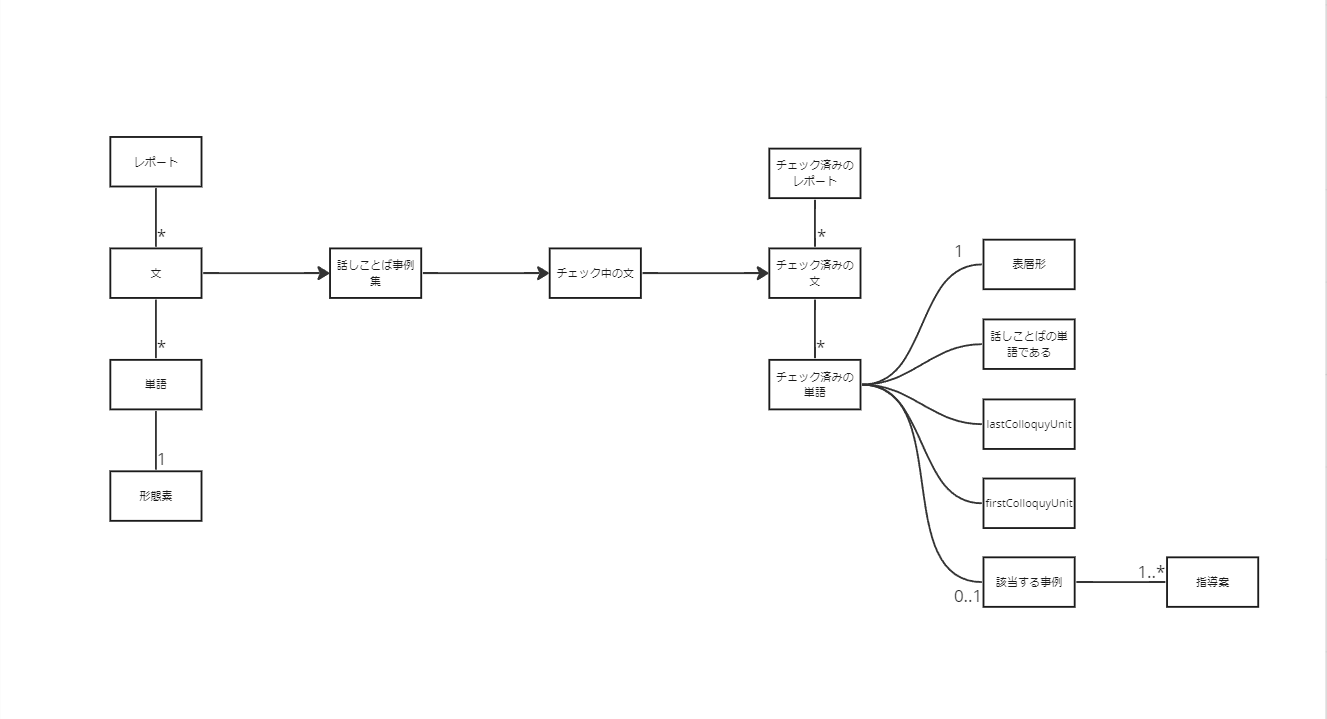
\includegraphics[width=1\linewidth]{image/kaizen2.png}
\caption{リファクタリングによるアーキテクチャの変化}
\label{fig:enter-label}
\end{figure}
2について、山下の論文内に存在する語をユビキタス言語として使用し、下に示す図4.2のように日本語の単位をモデリングに取り入れたことで、問題の解決方法の解釈のことであるメンタルモデルをプログラムコードに反映した。それにより、命名や構造に開発者の独自の解釈を用いていないプログラムコードへと改善した。
\begin{figure}[H]
\centering
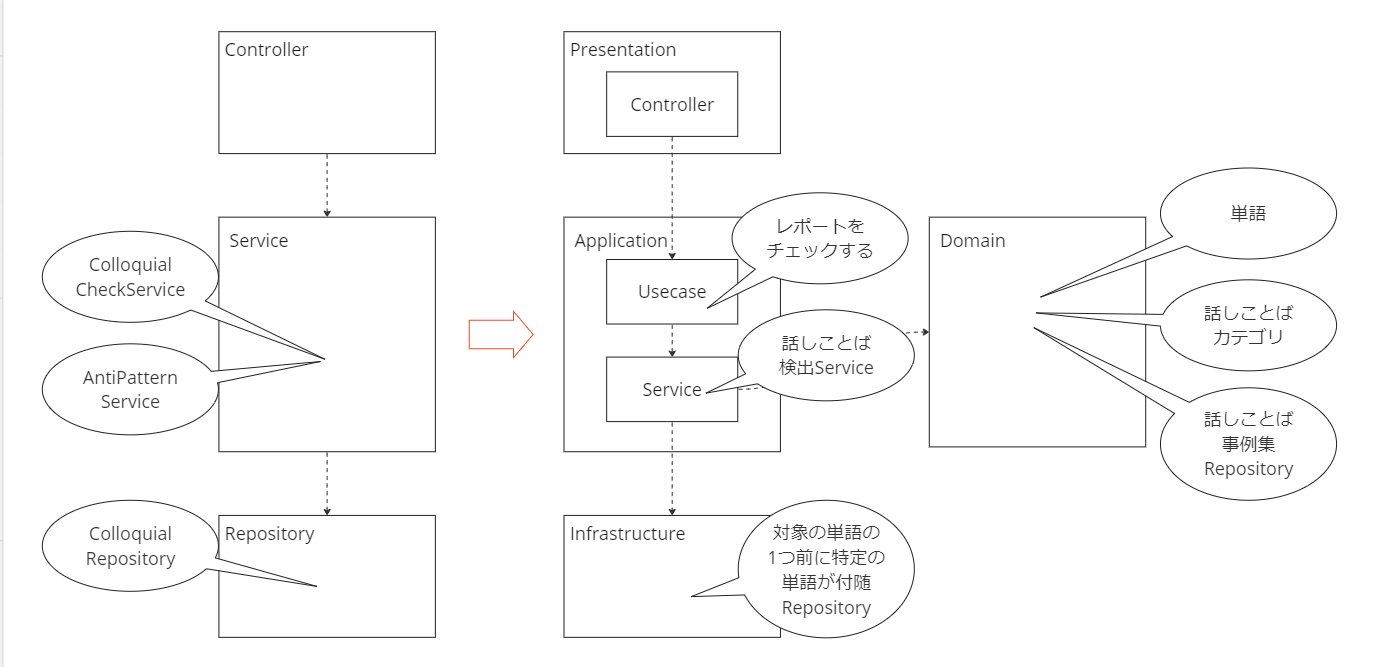
\includegraphics[width=1\linewidth]{image/kaizen1.png}
\caption{プログラムコードに反映したメンタルモデルの一部}
\label{fig:enter-label}
\end{figure}
3について、プログラムコードにテストコードを追加したことで、このシステムではどのような操作と結果が期待されているのか確認できるようになった。下の図4.3に示すようにテストケースの命名、入力と期待する出力にこういった観察可能な振る舞いを確認することができるようなプログラムコードに改善した。
\begin{figure}[H]
\centering
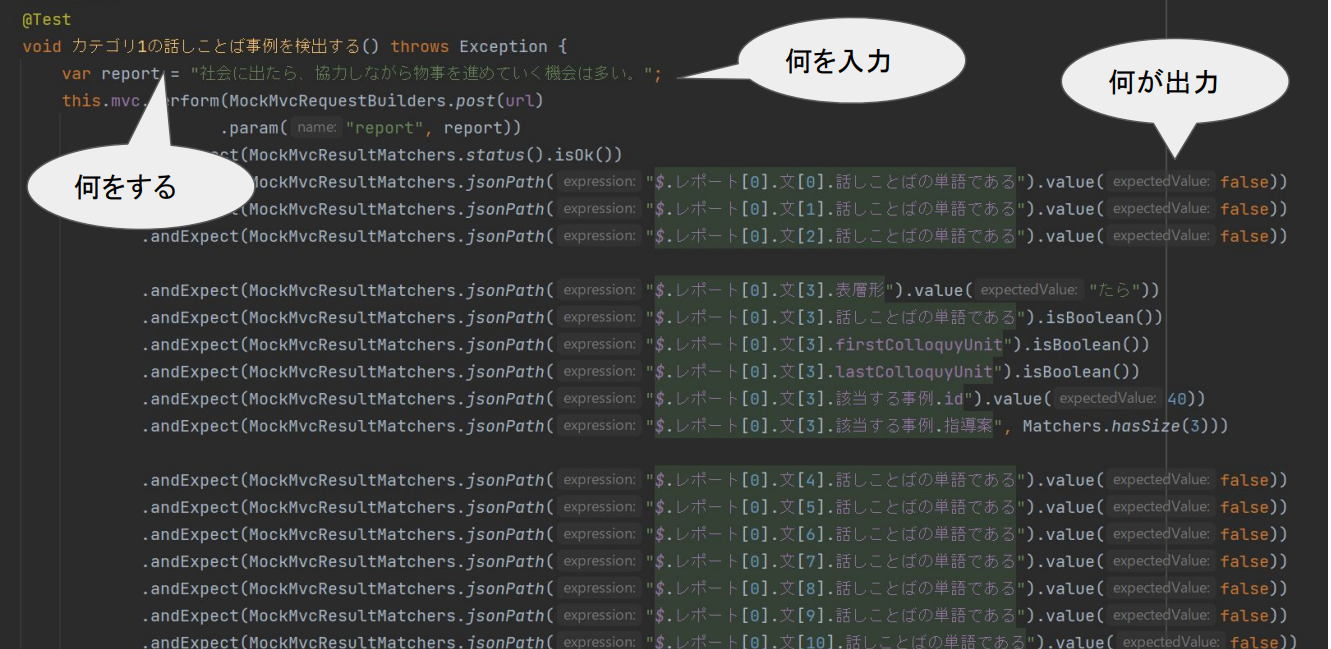
\includegraphics[width=1\linewidth]{image/kaizen3.png}
\caption{テストコードの例}
\label{fig:enter-label}
\end{figure}
\chapter{評価方法の検討}
\section{評価方法}
\subsection{責務を分けたコード}
責務を分けたコードとなっているか、凝集度を用いた定量評価を行う。凝集度とはクラス内のデータとロジックの関係性の強さを表す指標であり、クラス内に責務がどの程度集中しているか示すことができるものである。
\\ 凝集度を計測できるツールとしてYegor Bugayenkoが公開しているjPeekの5つの指標で計測する。5つの指標は以下の通りである。
\\
\begin{equation}
CAMC:
\frac{a}{kl}
\end{equation}
$a$ :メソッド内の型の数, $k$ :メソッドの数, $l$ :型の数
\begin{equation}
LCOM5:
\frac{a-kl}{l-kl}
\end{equation}
$a$ :メソッド内のattributesの数, $k$ :メソッドの数, $l$ : attributesの数
\begin{equation}
MMAC:
\frac{\sum^{i=l}_{i=1}{{x}_{i}{({x}_{i}-1})}}{lk(k-1)}
\end{equation}
$l$ : 型の数, $k$ : メソッドの数, ${x}_{i}$ : 戻り値が${i}$のメソッドの数
\begin{equation}
NHD:
1-\frac{2}{lk(k-1)}\sum^{l}_{j=1}{x}_{i}{(k-{x}_{i})}
\end{equation}

\begin{equation}
SCOM:
\frac{2}{m(m-1)}\sum^{m-1}_{i=1}\sum^{m}_{j=i+1}\frac{|{I}_{i}\cap{I}_{j}|}{min(|{I}_{i}|,|{I}_{j}|)}*\frac{|{I}_{i}\cup{I}_{j}|}{l}
\end{equation}
\\これらの指標でリファクタリング前後の凝集度を算出し、結果の比較を行う。
\subsection{共有されたメンタルモデルを反映させたコード}
リファクタリング前後のプログラムコードを文書化し、それを用いてドメインエキスパートにインタビューを行うことで、共有されたメンタルモデルが反映されたコードとなっているか定性評価を行う。
\\ 文書化にあたり、IDEであるintelliJでVanStudioが公開しているSequence Diagramというシーケンス図を生成するプラグインを利用する。生成したシーケンス図を用いて、メッセージを受け取るライフラインとメッセージの内容を「で」で繋げ、処理が行われる順番通りに番号を振ることで文書化する。この文書を用いてメンタルモデルが合っているかどうか、メンタルモデルが合っている部分はコードに直接メンタルモデルを表現できているかについて、ドメインエキスパートである山下にインタビューを行う。
\subsection{観察可能な振る舞いを確認できるコード}
テストコードを文書化し、それを用いてドメインエキスパートにインタビューを行うことで観察可能な振る舞いを確認できるコードとなっているか定性評価を行う。
\\ テストコードを記述したクラスの名前とテストケースの名前、assertで使用している入力、期待する出力を並べて文書を作成する。
\section{評価結果と考察}
\subsection{責務を分けたコード}
jPeekを用いて5つの指標について算出した結果を表5.1に示す。
\begin{table}[H]
\centering
\caption{jPeekによる算出結果}
\label{ttt}
\resizebox{\textwidth}{!}{%
\begin{tabular}{ | c | c | c | c | c | c | } \hline
~&CAMC&LCOM5&MMAC&NHD&SCOM\\ \hline\hline
リファクタリング前&0.97&0.50&0.50&9.32&0.50 \\ \hline
リファクタリング後&2.81&1.06&1.24&6.62&2.42\\ \hline
\end{tabular}%
}
\end{table}
CAMCはスコアが増加した。CAMCはクラス内の型の数が増加することでスコアが増加する。クラス内の型の数が増加した要因として、リファクタリングを経てプリミティブ型が減少したことが挙げられる。このことから、リファクタリング前にあった型がメンタルモデル独自の型に置き換わったと分かる。
\\ LCOM5はスコアが増加した。LCOM5はクラス内のattributesが減少することでスコアが増加する。クラス内のattributesが減少した要因として、クラス内で用いる変数やオブジェクトが限定的になったことが挙げられる。このことから、リファクタリングを経てクラス内の責務が減少したことが考えられる。
\\ MMACはスコアが増加した。MMACはメソッドの数に対する戻り値の型の種類が減少することでスコアが増加する。メソッドの数に対する戻り値の型の種類が減少した要因として、メソッドの数自体が減少したことが挙げられる。このことから、リファクタリングを経てクラス内の責務が減少したことが考えられる。
\\ NHDはスコアが減少した。NHDは型の数が減少することでスコアが増加する。クラス内の型の数が増加した要因として、リファクタリングを経てプリミティブ型が減少したことが挙げられる。このことから、リファクタリング前にあった型がメンタルモデル独自の型に置き換わったと分かる。
\\ SCOMはスコアが増加した。SCOMは類似したメソッドが増加することでスコアが増加する。類似したメソッドが増加した要因として、リファクタリングを経てメソッドに含まれるのattributesの種類が同じになったこと、濃度が均一になったことが挙げられる。このことから、リファクタリングを経てメソッド内の責務の量が均一になったと考えられる。
\subsection{共有されたメンタルモデルを反映させたコード}
シーケンス図を用いてリファクタリング前後のプログラムコードを文書化したものを以下の図5.1と図5.2に示す。
\begin{figure}[H]
\centering
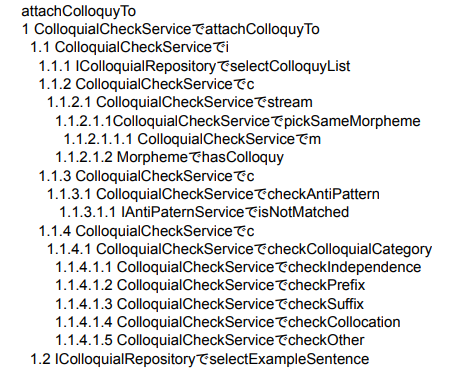
\includegraphics[width=1\linewidth]{image/modeiBe.png}
\caption{リファクタリング前のプログラムコードの文書化}
\label{fig:enter-label}
\end{figure}
\begin{figure}[H]
\centering
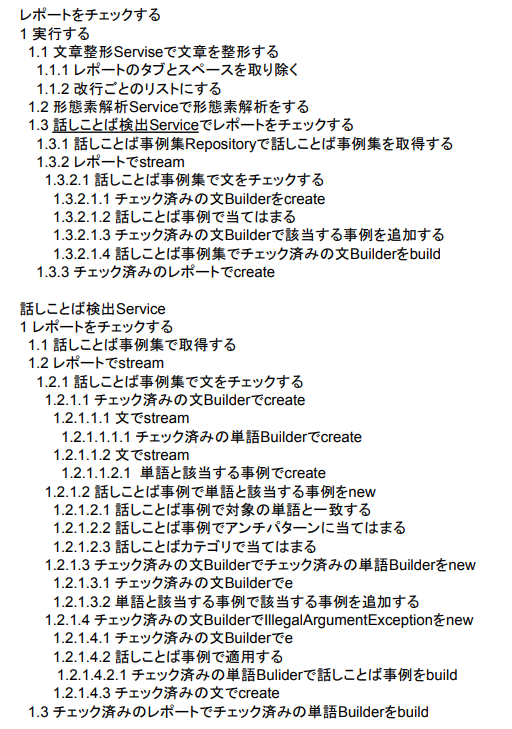
\includegraphics[width=1\linewidth]{image/modelAf.png}
\caption{リファクタリング後のプログラムコードの文書化}
\label{fig:enter-label}
\end{figure}
これらの文書を比較しリファクタリングを経て共有されたメンタルモデルを反映できているか、インタビューを行った。
\\ まず、「メンタルモデルが合っているか」について、リファクタリング後の方が山下の解釈に合っているという結果となった。そのように判断した理由として、文書の内容が日本語で記述されていることが挙げられた。「話しことば事例集は文をチェックするに文を渡したらチェック済みの文を出力する」という山下の論文には記述されていない処理の流れに関しても、山下の話しことば事例集の解釈の中にあったことが確認できた。
\\ 次に、「メンタルモデルが合っている部分はコードに直接メンタルモデルを表現できているか」について、「話しことば事例集」という山下の論文に合わせた表現を使用したことについては、分かりやすくなったという反応であった。ただし、「事例集」という表現を利用して「事例」という表現で記述した部分については文書だけでは伝わらず、口頭で説明を加えることで理解を得た。"C2Eins"などの表現をやめて、「対象の単語の一つ前に特定の単語が不随」などの山下の論文の言葉を使ったことについても、説明として分かりやすくなったという返答だった。また、streamやbuilder、iやeなどシステム開発上の入らざるを得ない言葉については理解を得られず、口頭で説明を加えた。文書化する際に用いた「で」という助詞にも正しい助詞であるのかと、疑問を抱いていた箇所があった。リファクタリング前の文書もリファクタリング後の文書もなんとなく理解できるが、リファクタリング前は英語で記述されているため、語句の理解に時間を要する結果となった。
\\ これらの結果から、ドメインモデルの構造や表現を利用したことで、共有されたメンタルモデルを部分的に反映することができたと考えられる。また、シーケンス図を基に作成した文書で開発者のメンタルモデルを共有することができることも明らかになった。ドメインエキスパートに「事例集」は伝わったが「事例」については疑問を抱いていたことから、ドメインモデルを吸い上げる際に使用するドキュメントに記載されていない言葉でプログラムコードを表現する場合には、開発者のメンタルモデルと異なる意味で捉えられる可能性があるので、ドメインエキスパートとの会話等で再定義するべきものがあると考えられる。本研究の評価では、シーケンス図のメッセージを特段選ばず、全てのメッセージを文書化したが、streamやbuilder, i, eといったシステム開発上の都合で存在しているメッセージに関しては、理解の妨げになっている様子も見られた。このことから、シーケンス図を用いてプログラムコードの文書化を行う際には、システム開発上の都合で存在しているメッセージは分かりやすい別の言葉で置き換えること、または置き換えた言葉との対応表を用意すること、または意図的に隠すこと等といった、メンタルモデルを共有しやすい文書となるよう考慮する必要がある。
\subsection{観察可能な振る舞いを確認できるコード}
テストコードを文書化したものを図5.3に示す。
\begin{figure}[H]
\centering
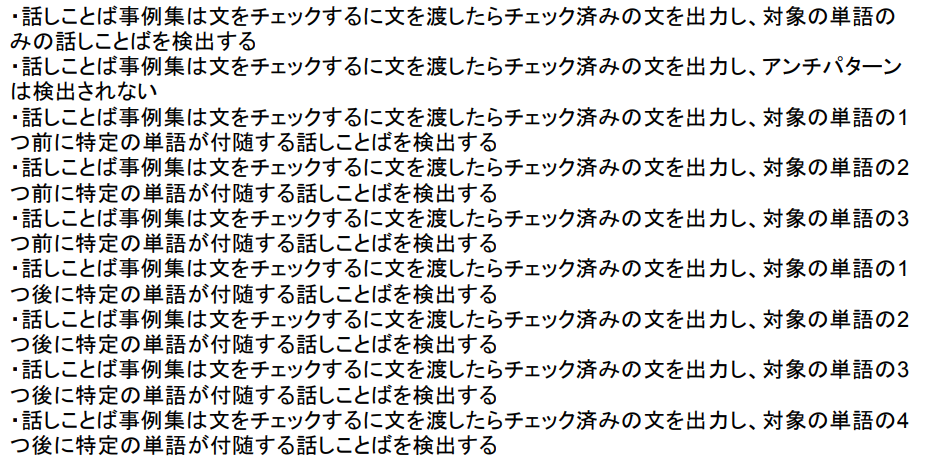
\includegraphics[width=1\linewidth]{image/hurumai.png}
\caption{テストコードの文書化}
\label{fig:enter-label}
\end{figure}
これを用いて、期待する操作と結果を確認できるかどうか、インタビューを行った。
\\ 結果としては箇条書き3つ目以降の「対象の単語の前後に特定の単語が不随する話しことば」について、期待する操作と結果として認識していなかったことが明らかになった。山下の論文では「対象の単語のみ」と「対象の単語の前に特定の単語が不随する」、「対象の単語の後に特定の単語が不随する」という言葉の記載がある。「特定の単語が付随するか」を判断する際に、「1つ前、2つ前、3つ前」や「1つ後、2つ後、3つ後、4つ後」といった特定の位置の単語を用いるものがあり、それをプログラムコードでは「対象の単語の前に特定の単語が不随する」、「対象の単語の後に特定の単語が不随する」という言葉に位置を示す数字を織り込んで表現していた。しかし、ドメインエキスパートはそれをインタビュー時に把握していなかった。
\\ 以上から、ドメインエキスパートが把握していないドメインに関する具体的な振る舞いについても、本評価で使用した文書を用いることで確認できることが明らかになった。また、箇条書き3つ目以降の振る舞いに関しては、ドメインエキスパートから観察可能ではなかったことも分かる。
\chapter{結論}
\section{まとめ}
複雑さの防止効果が高いシステム開発上の要素が判明した。また、その要素がプログラムコードに反映されているか評価する方法について、責務を分けたコードに関しては凝集度による評価、共有されたメンタルモデルを反映させたコードと観察可能な振る舞いを確認できるコードについてはプログラムコードをドキュメント化したものを用いてのインタビューにより評価できることが明らかになった。これにより、責務が分けられたコードであるか誰もが確認できる方法、メンタルモデルや観察可能な振る舞いを誰もが共有できる方法を実現できる可能性が見えたといえる。
\section{今後の課題}
\renewcommand{\bibname}{参考文献}
\addcontentsline{toc}{chapter}{参考文献}
\begin{thebibliography}{10}
\bibitem{haikei}「認知負荷を減らしたプログラミング学習支援に関する研究」石井 元規, 松本 慎平, 林 雄介, 平嶋 宗, 教育システム情報学会 2016年度学生研究発表会, 175-176
\bibitem{CyberZ}「良いコードとは何か」森 篤史, 2021年度 株式会社サイバーエージェント エンジニア新卒研修\url{https://note.com/cyberz_cto/n/n26f535d6c575#HPZ6C}
\bibitem{kireina}「動作するきれいなプログラムを継続的に記述していくための方策について」松田 俊寛, ITJ 2015.12 第16号, 54-59
\end{thebibliography}

\chapter*{謝辞}
\addcontentsline{toc}{chapter}{謝辞}
\end{document}
